\documentclass[a4paper,12pt]{article}
\usepackage[utf8]{inputenc}
\usepackage[T2A]{fontenc}
\usepackage[russian]{babel}
\usepackage{amsmath, amssymb, amsfonts}
\usepackage{graphicx}
\graphicspath{{../results/}{../}}
\usepackage{geometry}
\usepackage{hyperref}
\usepackage{float}
\usepackage{booktabs}
\usepackage{array}
\usepackage{subcaption}
\usepackage{algorithm}
\usepackage{algorithmic}

\geometry{a4paper, top=2cm, bottom=2cm, left=2.5cm, right=1.5cm}

% Перевод команд algorithmic
\renewcommand{\algorithmicrequire}{\textbf{Вход:}}
\renewcommand{\algorithmicensure}{\textbf{Выход:}}
\renewcommand{\algorithmicwhile}{\textbf{До тех пор, пока}}
\renewcommand{\algorithmicdo}{\textbf{цикл}}
\renewcommand{\algorithmicendwhile}{\textbf{конец цикла}}
\renewcommand{\algorithmicfor}{\textbf{Для}}
\renewcommand{\algorithmicforall}{\textbf{Для всех}}
\renewcommand{\algorithmicloop}{\textbf{Цикл}}
\renewcommand{\algorithmicrepeat}{\textbf{Повторять}}
\renewcommand{\algorithmicuntil}{\textbf{пока}}
\renewcommand{\algorithmicif}{\textbf{Если}}
\renewcommand{\algorithmicthen}{\textbf{то}}
\renewcommand{\algorithmicelse}{\textbf{иначе}}
\renewcommand{\algorithmicendif}{\textbf{конец если}}
\renewcommand{\algorithmicdo}{\textbf{делать}}
\renewcommand{\algorithmicendfor}{\textbf{конец цикла}}

\begin{document}
	
	% Титульный лист
	% Титульный лист
	\begin{titlepage}
		\begin{center}
			{\Large МОСКОВСКИЙ ГОСУДАРСТВЕННЫЙ УНИВЕРСИТЕТ \\ 
				имени М.В. ЛОМОНОСОВА}
			
			\vspace{0.5cm}
			{\Large МЕХАНИКО-МАТЕМАТИЧЕСКИЙ ФАКУЛЬТЕТ}
			
			\vspace{0.3cm}
			{\large Кафедра аэромеханики и газовой динамики}
			
			\vspace{3cm}
			
			{\Large \textbf{Задача по компьютерному практикуму}}
			
			\vspace{0.5cm}
			{\Large \textbf{Исследование дозвукового обтекания круглого цилиндра}}
			
			\vspace{0.5cm}
			{\large \textbf{на основе метода конформных отображений и полностью неявного метода}}
			
			\vspace{3cm}
			
			\begin{flushright}
				\large
				студент 5 курса \\
				Платонычев Иван Андреевич \\[1cm]
				Преподаватель по задаче: \\
				кандидат физико-математических наук \\
				Александр Николаевич Белоглазкин
			\end{flushright}
			
			\vspace{2cm}
			
			\begin{center}
				\large Москва \\
				\large 2026
			\end{center}
		\end{center}
	\end{titlepage}
	
	\newpage
	\tableofcontents
	\newpage
	
	\section{Постановка задачи}

\begin{figure}[h!]\centering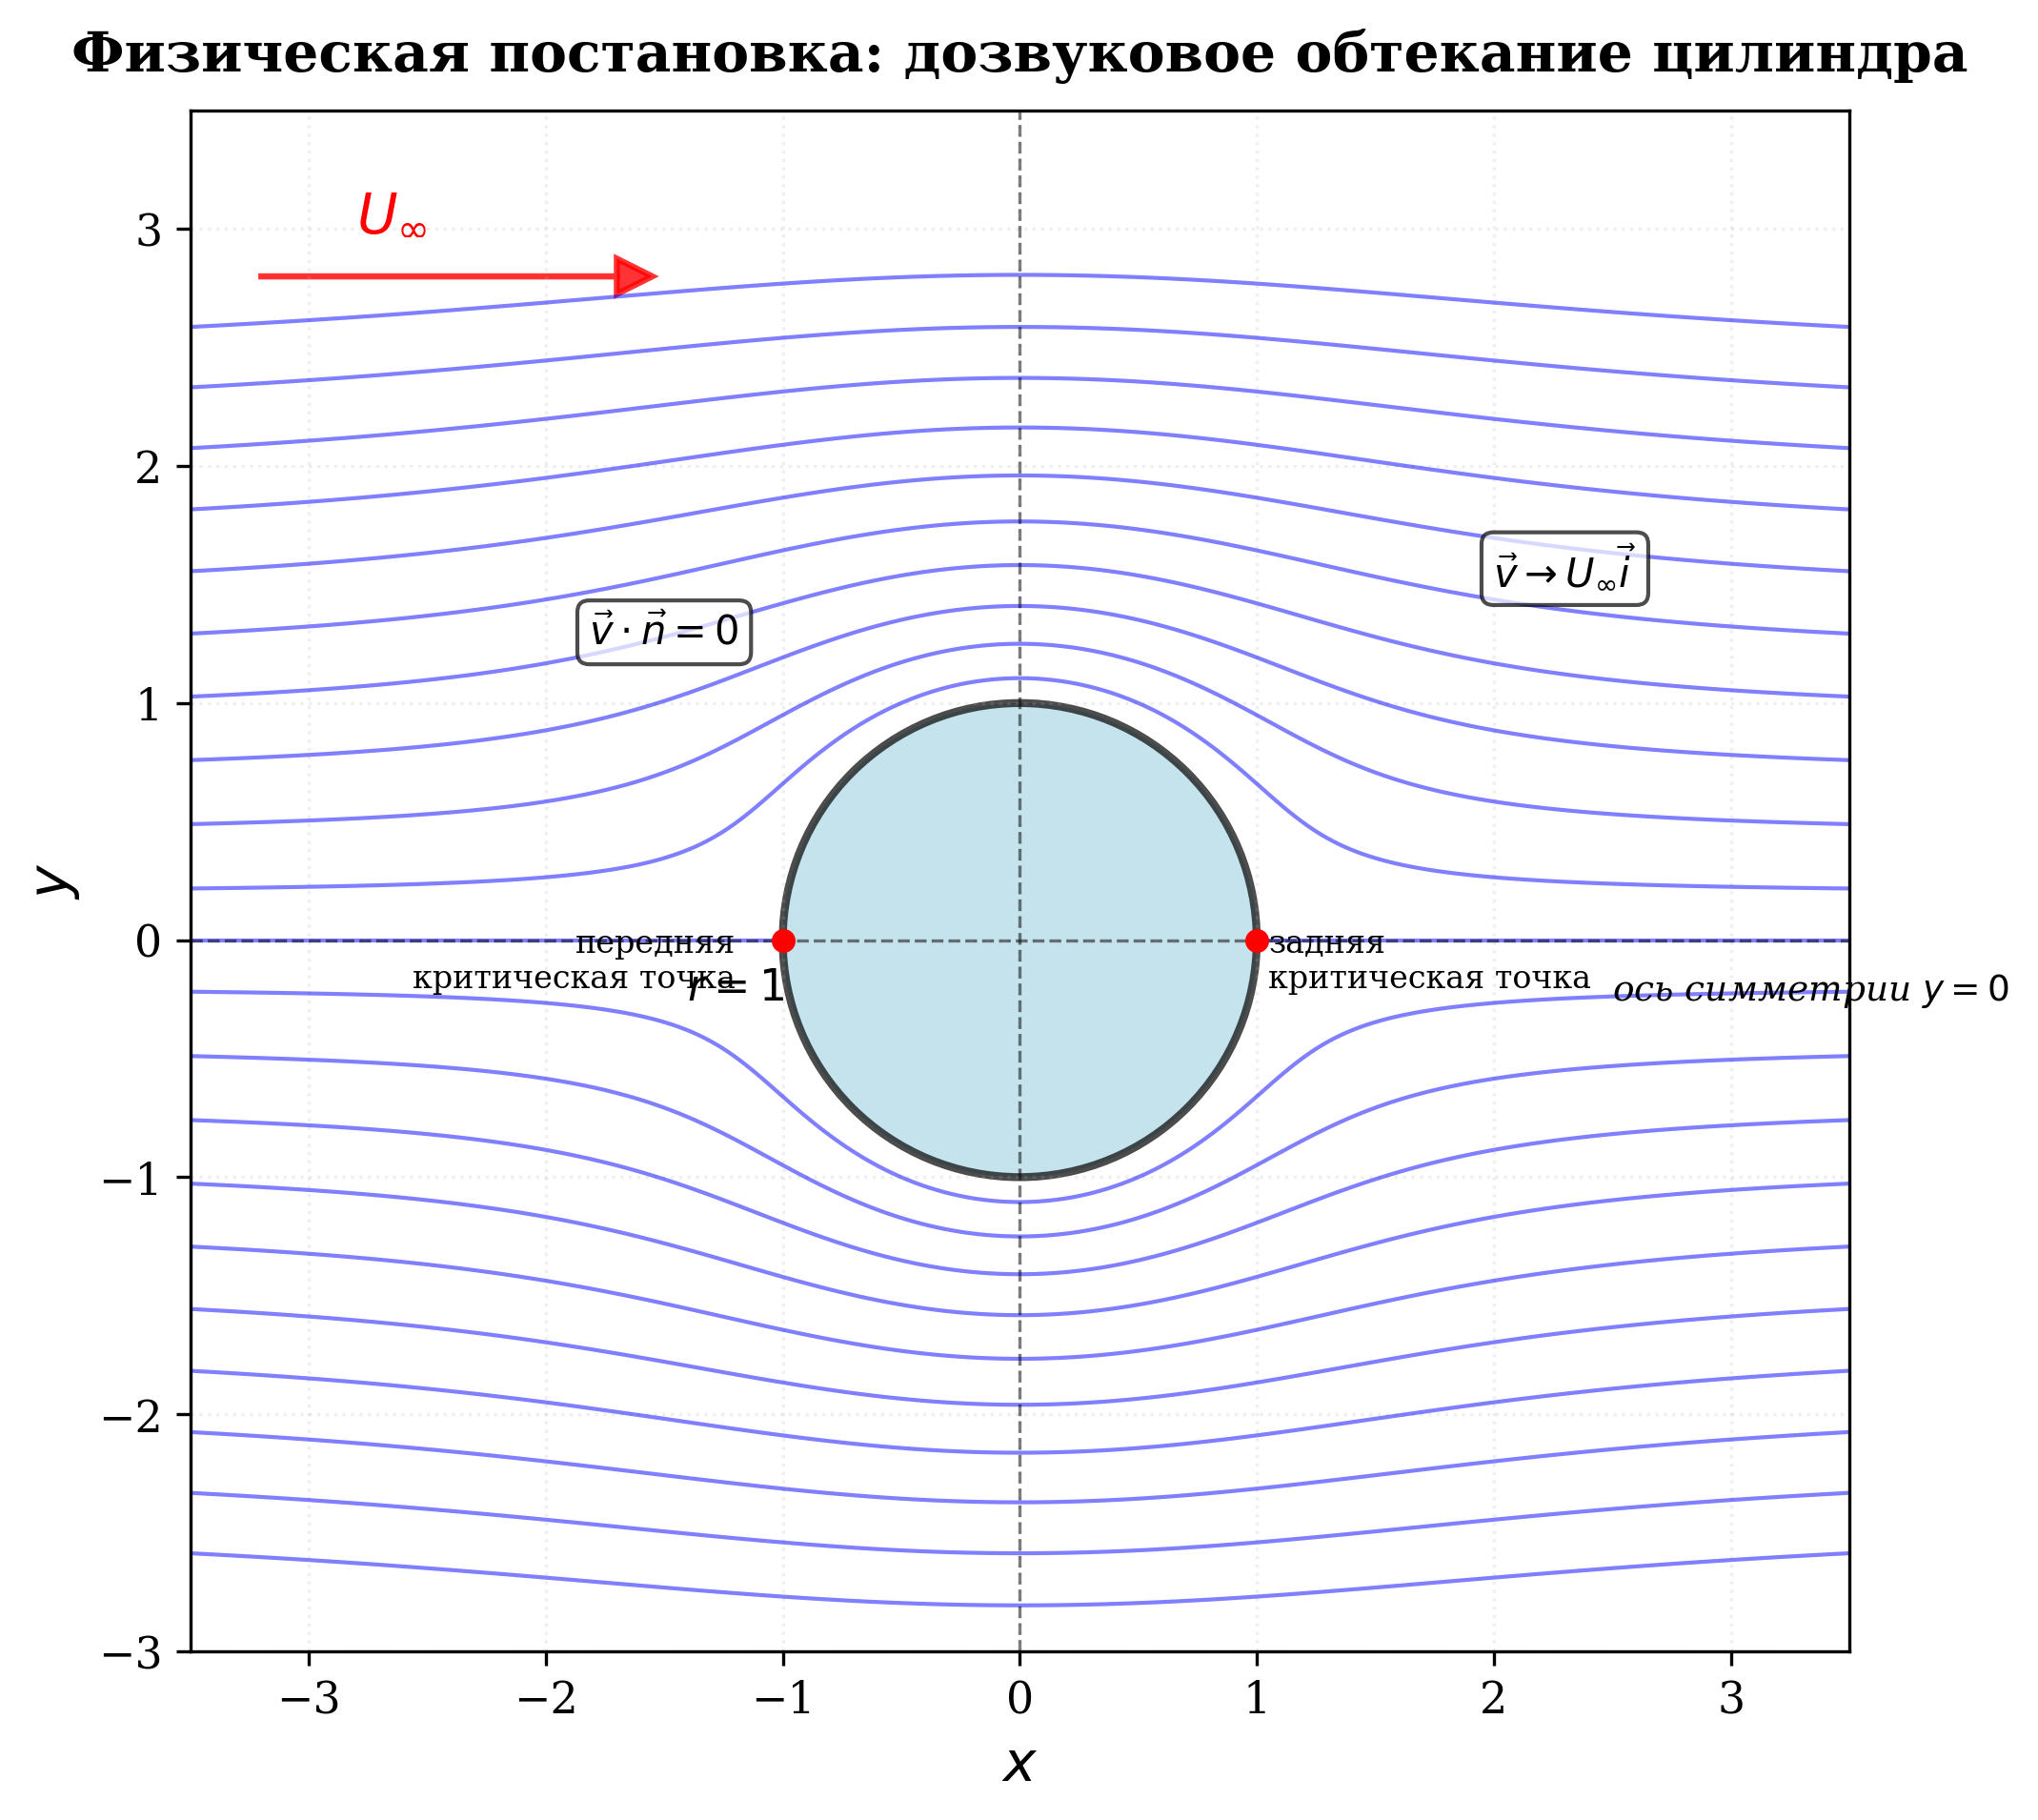
\includegraphics[width=0.4\textwidth]{1_physical_setup.png}\caption{Физическая постановка}\label{fig:setup}\end{figure}
	
	Рассматривается дозвуковое обтекание круглого цилиндра (рис. \ref{fig:setup}). В случае отсутствия завихренности стационарные двумерные уравнения Эйлера можно свести к нелинейному дифференциальному уравнению второго порядка в частных производных относительно потенциала скорости
	
	\[\vec{v} = \nabla \varphi.\]
	В декартовой системе координат имеем уравнение:
	
	\[
		\frac{\partial}{\partial x} \left( \rho \frac{\partial \varphi}{\partial x} \right) + \frac{\partial}{\partial y} \left( \rho \frac{\partial \varphi}{\partial y} \right) = 0,
	\]
	
	где плотность $\rho$ можно получить из условия изэнтропичности.
	
	На оси симметрии, на поверхности цилиндра задается условие непротекания
	
	
	

	\[\vec{v} \cdot \vec{n} = 0. \]	

	
	На больших расстояниях от цилиндра задается условие для невозмущенного потока
	
	
	\[ \vec{v}(r) \to U_{\infty} \vec{i} \quad \text{при} \quad r \to \infty.\]	
	
	
	В рамках данной постановки необходимо исследовать дозвуковое обтекание круглого цилиндра, используя конформное преобразование $\zeta = \ln z$, переводящее внешность единичной окружности на полуполосу $\xi \in [0, +\infty)$, $\eta \in [0, 2\pi]$.
	
	\textbf{Требуется}
	
	В рамках данной работы необходимо выполнить следующие задачи:
	
	\begin{enumerate}
		\item Вывести уравнения и соответствующие граничные условия в системе координат \((\xi, \eta)\).
		\item Составить разностную схему и решить ее с помощью ПНМ (Полностью Неявный Метод),
		сравнить данные по сходимости метода ПНМ с методом релаксации (неявную схема второго
		порядка по поперечной координате).
		\item В расчетной области для различных чисел Маха набегающего потока провести расчеты и сравнить распределение скорости и локального числа Маха.
		\item Исследовать зависимость результатов расчета от параметров сетки.
	\end{enumerate}
	
	\begin{thebibliography}{99}
		\bibitem{bai1961} Бай Ши-и, \textit{Введение в теорию течения сжимаемой жидкости}, ИЛ., М., 1961.
		\bibitem{buleev1959} Булеев Н.И. Численный метод решения двумерных уравнений диффузии // Атомная энергия, 1959, Том 6, № 3, С. 338–340.
		\bibitem{stone1968} Stone H.L. Iterative Solution of Implicit Approximations of Multidimensional Partial Differential Equations // SIAM Journal on Numerical Analysis, 1968, Vol. 5, No. 3, P. 530–558.
		\bibitem{pepper1977} D.W. Pepper, S.D. Harris, Fully Implicit Algorithms for Solving Partial Differential Equations // Journal of Fluids Engineering, 1977, 12, 781–783.
		\bibitem{beloglazkin1992} Белоглазкин А.Н., Шкадов В.Я. О влиянии проницаемости профиля на положение и интенсивность скачка при трансзвуковых скоростях // Вест. Моск. ун-та, сер. 1, математика, механика, 1992, № 5, С. 64–69.
	\end{thebibliography}
	\newpage

	\section{Уравнения Эйлера в размерном виде}
	
	Рассматривается стационарная задача, поэтому слагаемые, зависящие от времени, в уравнениях Эйлера опущены. Для описания течения сжимаемого газа используем систему уравнений Эйлера в размерном виде. Обозначим размерные величины со звездочкой $*$. 
	
	Уравнение неразрывности:
	\[
	\frac{\partial (\rho^* u^*)}{\partial x^*} + \frac{\partial (\rho^* v^*)}{\partial y^*} = 0.
	\]
	
	Уравнения движения (компоненты):
	\[
	\rho^* \left( u^* \frac{\partial u^*}{\partial x^*} + v^* \frac{\partial u^*}{\partial y^*} \right) = -\frac{\partial p^*}{\partial x^*},
	\]
	\[
	\rho^* \left( u^* \frac{\partial v^*}{\partial x^*} + v^* \frac{\partial v^*}{\partial y^*} \right) = -\frac{\partial p^*}{\partial y^*}.
	\]
	
	Уравнение энергии для изэнтропического течения:
	\[
	\frac{p^*}{\rho^{*\gamma}} = \text{const},
	\]
	где $\gamma$ — показатель адиабаты.
	
	Для стационарного безвихревого течения существует потенциал скорости $\varphi^*$, такой что:
	\[
	u^* = \frac{\partial \varphi^*}{\partial x^*}, \quad v^* = \frac{\partial \varphi^*}{\partial y^*}.
	\]
	
	Тогда уравнение неразрывности принимает вид:
	\[
	\frac{\partial}{\partial x^*} \left( \rho^* \frac{\partial \varphi^*}{\partial x^*} \right) + \frac{\partial}{\partial y^*} \left( \rho^* \frac{\partial \varphi^*}{\partial y^*} \right) = 0.
	\]
	
	Из условия изэнтропичности и интеграла Бернулли для безвихревого течения:
	\[
	\frac{\gamma}{\gamma-1} \frac{p^*}{\rho^*} + \frac{1}{2} \left( \frac{\partial \varphi^*}{\partial x^*} \right)^2 + \frac{1}{2} \left( \frac{\partial \varphi^*}{\partial y^*} \right)^2 = 
	\frac{\gamma}{\gamma-1} \frac{p_\infty}{\rho_\infty} + \frac{1}{2} U_\infty^2.
	\]
	
	\subsection{Граничные условия в размерной постановке}
	
	\subsubsection{Условие непротекания на поверхности цилиндра}
	На поверхности цилиндра радиуса $R$ (в размерной форме) задается условие непротекания:
	\[
	\vec{v}^* \cdot \vec{n} = 0 \quad \text{при} \quad r^* = R,
	\]
	где $\vec{n}$ — единичный вектор нормали к поверхности цилиндра.
	
	В полярных координатах $(r^*, \theta)$ это условие записывается как:
	\[
	\frac{\partial \varphi^*}{\partial r^*} = 0 \quad \text{при} \quad r^* = R.
	\]
	
	\subsubsection{Условие на бесконечности}
	На больших расстояниях от цилиндра поток невозмущенный:
	\[
	\vec{v}^*(r^*) \to U_\infty^* \vec{i} \quad \text{при} \quad r^* \to \infty,
	\]
	где $U_\infty^*$ — скорость набегающего потока. В терминах потенциала скорости:
	\[
	\varphi^* \to U_\infty^* x^* \quad \text{при} \quad r^* \to \infty.
	\]

	\section{Безразмерная постановка задачи}
	
	Для приведения системы уравнений Эйлера к безразмерному виду используем $\pi$-теорему теории размерности. В качестве основных масштабов выберем:
	\begin{itemize}
		\item Масштаб длины: $L = R$ — радиус цилиндра,
		\item Масштаб скорости: $U_\infty$ — скорость набегающего потока,
		\item Масштаб плотности: $\rho_\infty$ — плотность невозмущенного потока,
		\item Масштаб давления: $\rho_\infty U_\infty^2$.
	\end{itemize}
	
	Введем следующие безразмерные переменные:
	\[
	x = \frac{x^*}{L}, \quad y = \frac{y^*}{L}, \quad \varphi = \frac{\varphi^*}{U_\infty L}, \quad \rho = \frac{\rho^*}{\rho_\infty}, \quad p = \frac{p^*}{\rho_\infty U_\infty^2} \\
	\quad u = \frac{u^*}{U_\infty}, \quad a = \frac{a^*}{a_\infty}\quad M_{loc} = \frac{q}{a}\cdot M_\infty.
	\]
	
	Размер расчетной области задан величиной $R_\infty = 20$. Основным варьируемым параметром задачи является число Маха набегающего потока $M_\infty$.
	
	\subsection{Безразмерные уравнения Эйлера}
	
	\subsubsection{Уравнение неразрывности}
	\[
	\frac{\partial (\rho u)}{\partial x} + \frac{\partial (\rho v)}{\partial y} = 0.
	\]
	
	\subsubsection{Уравнения движения (компоненты)}
	\[
	\rho \left( u \frac{\partial u}{\partial x} + v \frac{\partial u}{\partial y} \right) = -\frac{\partial p}{\partial x},
	\]
	\[
	\rho \left( u \frac{\partial v}{\partial x} + v \frac{\partial v}{\partial y} \right) = -\frac{\partial p}{\partial y}.
	\]
	
	\subsubsection{Уравнение для потенциала скорости}
	При условии безвихревости течения $\nabla \times \vec{v} = 0$ существует потенциал скорости $\vec{v} = \nabla \varphi$. Уравнение неразрывности в безразмерной форме принимает вид:
	\[
	\frac{\partial}{\partial x} \left( \rho \frac{\partial \varphi}{\partial x} \right) + \frac{\partial}{\partial y} \left( \rho \frac{\partial \varphi}{\partial y} \right) = 0.
	\]
	
	\subsubsection{Уравнение изэнтропичности и связь плотности с потенциалом}
	
	Из интеграла Бернулли для безвихревого изэнтропического течения:
	\[
	\frac{\gamma}{\gamma-1} \frac{p}{\rho} + \frac{1}{2} (u^2 + v^2) = \frac{1}{(\gamma-1)M^2_\infty} + \frac{1}{2}.
	\]
	
	С учетом изэнтропического соотношения $p / \rho^\gamma = \text{const}$ и переходя к безразмерным переменным, получим:
	\[
	\rho = \left[ 1 + \frac{\gamma-1}{2} M_\infty^2 \left( 1 - (u^2 + v^2) \right) \right]^{\frac{1}{\gamma-1}},
	\]
	где $M_\infty = U_\infty / a_\infty$ — число Маха набегающего потока, $a_\infty = \sqrt{\gamma p_\infty / \rho_\infty}$ — скорость звука в невозмущенном потоке.
	
	В терминах потенциала скорости:
	\[
	u = \frac{\partial \varphi}{\partial x}, \quad v = \frac{\partial \varphi}{\partial y},
	\]
	\[
	q^2 = u^2 + v^2 = \left( \frac{\partial \varphi}{\partial x} \right)^2 + \left( \frac{\partial \varphi}{\partial y} \right)^2.
	\]
	
	Таким образом, плотность выражается через потенциал скорости:
	\begin{equation}
		\boxed{\rho = \left[ 1 + \frac{\gamma-1}{2} M_\infty^2 \left( 1 - \left( \frac{\partial \varphi}{\partial x} \right)^2 - \left( \frac{\partial \varphi}{\partial y} \right)^2 \right) \right]^{\frac{1}{\gamma-1}}}
		\label{eq:density}
	\end{equation}
	
	\subsection{Безразмерные граничные условия}
	
	\subsubsection{Условие непротекания на поверхности цилиндра}
	На поверхности цилиндра $r = 1$ (в безразмерных координатах) нормальная компонента скорости равна нулю:
	\[
	\vec{v} \cdot \vec{n} = 0 \quad \text{при} \quad r = 1.
	\]
	В полярных координатах это соответствует условию:
	\[
	\frac{\partial \varphi}{\partial r} = 0 \quad \text{при} \quad r = 1.
	\]
	
	\subsubsection{Условие на бесконечности}
	На больших расстояниях от цилиндра поток полагается невозмущенным (условие Дирихле):
	\[
	\varphi \to x = r \cos \theta \quad \text{при} \quad r \to \infty.
	\]
	
	
	
	%%%%%%%%%%%%%%%%%%%%%%%%%%%%%%%%%

	\section{Преобразование координат и вывод уравнений в системе \texorpdfstring{$(\xi, \eta)$}{(xi, eta)}}
	
	\subsection{Конформное преобразование}
	
	Введем комплексную переменную $z = x + iy$. Конформное отображение (рис. \ref{fig:mapping}), переводящее внешность единичной окружности в полуполосу, имеет вид:
	\begin{equation}
		\zeta = \ln z = \xi + i\eta,
	\end{equation}
	где $\xi = \ln |z| = \ln r$, $\eta = \arg z = \theta$.
	
	При таком преобразовании:
	\begin{itemize}
		\item Внешность единичной окружности $|z| \ge 1$ отображается в полуполосу $\xi \in [0, +\infty)$, $\eta \in [0, 2\pi)$.
		\item Поверхность цилиндра $|z| = 1$ отображается в линию $\xi = 0$.
		\item Бесконечно удаленная точка $|z| \to \infty$ отображается в $\xi \to +\infty$.
	\end{itemize}
	
	\subsection{Уравнение для потенциала скорости в координатах \texorpdfstring{$(\xi, \eta)$}{(xi, eta)}}
	В декартовых координатах уравнение для потенциала скорости имеет вид:
	\[
	\frac{\partial}{\partial x} \left( \rho \frac{\partial \varphi}{\partial x} \right) + \frac{\partial}{\partial y} \left( \rho \frac{\partial \varphi}{\partial y} \right) = 0.
	\]
	
	Для конформного отображения $w = f(z)$ оператор Лапласа преобразуется как:
	\[
	\frac{\partial^2}{\partial x^2} + \frac{\partial^2}{\partial y^2} = |f'(z)|^2 \left( \frac{\partial^2}{\partial \xi^2} + \frac{\partial^2}{\partial \eta^2} \right).
	\]
	
	В нашем случае $f(z) = \ln z$, следовательно:
	\[
	f'(z) = \frac{1}{z} = e^{-\zeta} = e^{-\xi} e^{-i\eta}, \quad |f'(z)| = e^{-\xi}.
	\]
	
	Метрический коэффициент (якобиан) преобразования:
	\[
	J = |f'(z)|^{-2} = e^{2\xi}.
	\]
	
	Уравнение неразрывности в криволинейных координатах имеет вид:
	\[
	\frac{\partial}{\partial \xi} \left( \rho \frac{\partial \varphi}{\partial \xi} \right) + \frac{\partial}{\partial \eta} \left( \rho \frac{\partial \varphi}{\partial \eta} \right) = 0,
	\]
	где использовано соотношение $\sqrt{g} = |f'(z)|^{-1} = e^{\xi}$ и тот факт, что для конформного отображения коэффициенты Ламэ равны. Более подробный вывод приведен в Приложении.
	
	Окончательное уравнение в координатах $(\xi, \eta)$:
	\begin{equation}
		\boxed{\frac{\partial}{\partial \xi} \left( \rho \frac{\partial \varphi}{\partial \xi} \right) + \frac{\partial}{\partial \eta} \left( \rho \frac{\partial \varphi}{\partial \eta} \right) = 0}
	\end{equation}
	
	\subsection{Выражение для плотности через потенциал скорости}
	Из интеграла Бернулли и условия изэнтропичности связь между плотностью и скоростью имеет вид:
	\[
	\rho = \left[ 1 + \frac{\gamma-1}{2} M_\infty^2 \left( 1 - q^2 \right) \right]^{\frac{1}{\gamma-1}},
	\]
	где $q^2 = u^2 + v^2$ — квадрат модуля скорости.
	
	В координатах $(\xi, \eta)$ компоненты физической скорости выражаются через потенциал:
	\[
	u = \frac{\partial \varphi}{\partial x} = e^{-\xi} \left( \cos\eta \frac{\partial \varphi}{\partial \xi} - \frac{\sin\eta}{e^{\xi}} \frac{\partial \varphi}{\partial \eta} \right), \quad
	v = \frac{\partial \varphi}{\partial y} = e^{-\xi} \left( \sin\eta \frac{\partial \varphi}{\partial \xi} + \frac{\cos\eta}{e^{\xi}} \frac{\partial \varphi}{\partial \eta} \right).
	\]
	Квадрат скорости:
	\[
	q^2 = u^2 + v^2 = e^{-2\xi} \left[ \left( \frac{\partial \varphi}{\partial \xi} \right)^2 + \left( \frac{\partial \varphi}{\partial \eta} \right)^2 \right].
	\]
	
	\subsection{Граничные условия в координатах \texorpdfstring{$(\xi, \eta)$}{(xi, eta)}}
	
	\subsubsection{Условие на поверхности цилиндра \texorpdfstring{($\xi = 0$)}{(xi = 0)}}
	На поверхности цилиндра $\xi = 0$ (твердая стенка) потенциал скорости $\varphi$ должен удовлетворять условию непротекания $\frac{\partial \varphi}{\partial \xi} = 0$. В численной реализации это соответствует центрально-разностной аппроксимации второго порядка, при которой значения в фиктивных узлах за стенкой определяются как:
	\[
	\varphi_{-1,j} = \varphi_{1,j}.
	\]
	
	\subsubsection{Условие на бесконечности \texorpdfstring{($\xi \to \infty$)}{(xi -> inf)}}
	При $\xi \to \infty$ потенциал скорости стремится к потенциалу невозмущенного потока (условие Дирихле):
	\[
	\varphi \to e^{\xi} \cos \eta \quad \text{при} \quad \xi \to \infty.
	\]
	
	\subsubsection{Условие на нижней и вехней границе}
	\[
	\varphi_{i,-1} = \varphi_{i,1}. \quad \varphi_{i,N_{\eta} -1} = \varphi_{i,N_{\eta} +1}
	\]
	%%%%%%%%%%%%%%%%%%%%%%%%%%%%%%%
	%%%%%%%%%%%%%%%%%%%%%%55	
	
	\begin{figure}[H]
	\centering
	
\includegraphics[width=0.6\textwidth]{stencil_scheme.png}
	\caption{Разностная схема и шаблоны в расчетной области $(\xi, \eta)$. Показаны модификации шаблонов на границах: для твердой стенки ($\xi=0$), оси симметрии ($\eta=0, \pi$) и узлов перед бесконечностью.}
	\label{fig:stencil}
\end{figure}

	\input{sections/5_pnm.tex}
	\section{Метод последовательной верхней релаксации по строкам (SLOR)}
	
	В качестве альтернативного численного метода решения уравнения для потенциала используется метод последовательной верхней релаксации по строкам (Successive Line Over-Relaxation). Основная идея метода заключается в одновременном решении значений потенциала для всех узлов вдоль одной строки сетки ($\eta = \text{const}$). 
	
	\subsection{Шаблон разностной схемы}
	
	Для реализации метода SLOR исходное пятиточечное уравнение в узле $(i,j)$ разделяется на неявную часть (вдоль текущей строки $j$) и явную часть (соседние строки $j-1$ и $j+1$):
	\begin{equation}
		\underbrace{A_i \varphi_{i-1,j} + B_i \varphi_{i,j} + C_i \varphi_{i+1,j}}_{\text{Неявная часть (строка } j\text{)}} = \underbrace{D_i}_{\text{Явная часть (соседние строки)}}
	\end{equation}
	Шаблон схемы можно представить следующим образом:
	\begin{equation*}
		\begin{matrix}
			& \varphi_{i,j+1}^{(n)} & \\
			& \uparrow & \\
			\varphi_{i-1,j}^{(n+1)} \leftarrow & \mathbf{\varphi_{i,j}^{(n+1)}} & \rightarrow \varphi_{i+1,j}^{(n+1)} \\
			& \downarrow & \\
			& \varphi_{i,j-1}^{(n+1)} & 
		\end{matrix}
	\end{equation*}
	Здесь значения на текущей строке $j$ и на уже обработанной строке $j-1$ берутся с новой итерации $(n+1)$, а значение на строке $j+1$ — с предыдущей итерации $(n)$.
	
	\subsection{Формирование трехдиагональной системы}
	На текущей итерации $n$ для каждой строки $j = 0, \dots, N_\eta$ решается система уравнений относительно неизвестных $\varphi_{i,j}$:
	\begin{equation}
		A_i \varphi_{i-1,j} + B_i \varphi_{i,j} + C_i \varphi_{i+1,j} = D_i,
		\label{eq:slor_tridiag}
	\end{equation}
	где значения в соседних строках ($j-1$ и $j+1$) считаются известными. При этом для строки $j-1$ используются уже обновленные на текущей итерации значения $\varphi_{i,j-1}^{(n+1)}$, а для строки $j+1$ — значения с предыдущей итерации $\varphi_{i,j+1}^{(n)}$.
	
	Коэффициенты для внутренних узлов ($i \in [1, N_\xi-1], j \in [1, N_\eta-1]$):
	\begin{itemize}
		\item $A_i = \displaystyle -\frac{\rho_{i-1/2,j}}{\Delta \xi^2}$
		\item $C_i = \displaystyle -\frac{\rho_{i+1/2,j}}{\Delta \xi^2}$
		\item $B_i = \displaystyle \frac{\rho_{i+1/2,j} + \rho_{i-1/2,j}}{\Delta \xi^2} + \frac{\rho_{i,j+1/2} + \rho_{i,j-1/2}}{\Delta \eta^2}$
		\item $D_i = \displaystyle \frac{\rho_{i,j+1/2} \varphi_{i,j+1} + \rho_{i,j-1/2} \varphi_{i,j-1}}{\Delta \eta^2}$
	\end{itemize}
	
	\subsection{Учет граничных условий}
	
	Для реализации граничных условий в узлах, лежащих на границах расчетной области, используются модифицированные коэффициенты и уравнения.
	
	\begin{enumerate}
		\item \textbf{Точки на поверхности цилиндра ($i=0$, условие Неймана):} 
		Используется условие непротекания $\varphi_{-1,j} = \varphi_{1,j}$. Это приводит к занулению коэффициента $A_0$ и модификации $B_0, C_0$:
		\begin{itemize}
			\item \textit{Граничные точки $i=0, j \in [1, N_\eta-1]$:}
			\[ A_0 = 0, \quad B_0 = \frac{2\rho_{1/2,j}}{\Delta \xi^2} + \frac{\rho_{0,j+1/2} + \rho_{0,j-1/2}}{\Delta \eta^2}, \quad C_0 = -\frac{2\rho_{1/2,j}}{\Delta \xi^2} \]
			\[ D_0 = \frac{\rho_{0,j+1/2} \varphi_{0,j+1} + \rho_{0,j-1/2} \varphi_{0,j-1}}{\Delta \eta^2} \]
			Уравнение принимает вид: $B_0 \varphi_{0,j} + C_0 \varphi_{1,j} = D_0$.
			
			\item \textit{Угловая точка $i=0, j=0$ (пересечение с нижней симметрией):}
			\[ A_0 = 0, \quad B_0 = \frac{2\rho_{1/2,0}}{\Delta \xi^2} + \frac{2\rho_{0,1/2}}{\Delta \eta^2}, \quad C_0 = -\frac{2\rho_{1/2,0}}{\Delta \xi^2}, \quad D_0 = \frac{2\rho_{0,1/2} \varphi_{0,1}}{\Delta \eta^2} \]
			Уравнение принимает вид: $B_0 \varphi_{0,0} + C_0 \varphi_{1,0} = D_0$.
			
			\item \textit{Угловая точка $i=0, j=N_\eta$ (пересечение с верхней симметрией):}
			\[ A_0 = 0, \quad B_0 = \frac{2\rho_{1/2,N_\eta}}{\Delta \xi^2} + \frac{2\rho_{0,N_\eta-1/2}}{\Delta \eta^2}, \quad C_0 = -\frac{2\rho_{1/2,N_\eta}}{\Delta \xi^2}, \quad D_0 = \frac{2\rho_{0,N_\eta-1/2} \varphi_{0,N_\eta-1}}{\Delta \eta^2} \]
			Уравнение принимает вид: $B_0 \varphi_{0,N_\eta} + C_0 \varphi_{1,N_\eta} = D_0$.
		\end{itemize}

		\item \textbf{Точки на линиях симметрии ($j=0$ и $j=N_\eta$, $i \in [1, N_\xi-1]$):} 
		Используется условие $\varphi_{i,-1} = \varphi_{i,1}$ (или аналогично для верхней границы), что приводит к удвоению потока по $\eta$:
		\begin{itemize}
			\item \textit{Нижняя линия симметрии ($j=0$):}
			\[ B_i = \frac{\rho_{i+1/2,0} + \rho_{i-1/2,0}}{\Delta \xi^2} + \frac{2\rho_{i,1/2}}{\Delta \eta^2}, \quad D_i = \frac{2\rho_{i,1/2} \varphi_{i,1}}{\Delta \eta^2} \]
			Уравнение для узла $(i,0)$ сохраняет трехдиагональный вид: 
			
			$A_i \varphi_{i-1,0} + B_i \varphi_{i,0} + C_i \varphi_{i+1,0} = D_i$.
			\item \textit{Верхняя линия симметрии ($j=N_\eta$):}
			\[ B_i = \frac{\rho_{i+1/2,N_\eta} + \rho_{i-1/2,N_\eta}}{\Delta \xi^2} + \frac{2\rho_{i,N_\eta-1/2}}{\Delta \eta^2}, \quad D_i = \frac{2\rho_{i,N_\eta-1/2} \varphi_{i,N_\eta-1}}{\Delta \eta^2} \]
			Уравнение для узла $(i,N_\eta)$ имеет вид: $A_i \varphi_{i-1,N_\eta} + B_i \varphi_{i,N_\eta} + C_i \varphi_{i+1,N_\eta} = D_i$.
		\end{itemize}

		\item \textbf{Внешняя граница ($i=N_\xi$, условие Дирихле):} 
		Значение потенциала фиксировано $\varphi_{N_\xi,j} = \varphi_{N_\xi,j}^\infty$. В системе для узла $i=N_\xi-1$ это учитывается переносом слагаемого в правую часть:
		\[ C_{N_\xi-1} = 0, \quad D_{N_\xi-1}^{new} = D_{N_\xi-1}^{old} - C_{N_\xi-1}^{old} \cdot \varphi_{N_\xi,j}^\infty \]
		Уравнение для последнего расчетного узла в строке: 
		
		$A_{N_\xi-1} \varphi_{N_\xi-2,j} + B_{N_\xi-1} \varphi_{N_\xi-1,j} = D_{N_\xi-1}$.

	\end{enumerate}
	
	\subsection{Релаксация}
	
	После нахождения промежуточного решения $\tilde{\varphi}_{i,j}$ из трехдиагональной системы, окончательное значение на итерации $n+1$ вычисляется с параметром сверхрелаксации $\omega$:
	\begin{equation}
		\varphi_{i,j}^{(n+1)} = (1 - \omega) \varphi_{i,j}^{(n)} + \omega \tilde{\varphi}_{i,j}
	\end{equation}
	Оптимальное значение $\omega$ для данной задачи обычно находится в диапазоне $1.5 \dots 1.8$.

	\section{Вычисление физических величин}
	
	После нахождения потенциала скорости $\varphi(\xi, \eta)$ в расчетной области производится расчет физических характеристик потока.
	
	Связь между расчетными $(\xi, \eta)$ и физическими $(x, y)$ координатами:
	\begin{equation}
		x = e^\xi \cos \eta, \quad y = e^\xi \sin \eta.
	\end{equation}
	
	Квадрат модуля безразмерной скорости в каждой точке вычисляется через производные потенциала:
	\begin{equation}
		q^2 = e^{-2\xi} \left[ \left( \frac{\partial \varphi}{\partial \xi} \right)^2 + \left( \frac{\partial \varphi}{\partial \eta} \right)^2 \right].
	\end{equation}
	
	Локальное число Маха $M_{loc}$ определяется как отношение скорости к локальной скорости звука:
	\begin{equation}
		M_{loc} = \frac{q \cdot M_\infty}{a}, \quad a^2 = 1 + \frac{\gamma-1}{2} (1 - q^2) M_\infty^2.
	\end{equation}
	
	Коэффициент давления $C_p$ рассчитывается по формуле для изэнтропического потока:
	\begin{equation}
		C_p = \frac{2}{\gamma M_\infty^2} \left( \rho^\gamma - 1 \right), \quad \text{где } \rho = \left[ 1 + \frac{\gamma-1}{2} M_\infty^2 (1 - q^2) \right]^{\frac{1}{\gamma-1}}.
	\end{equation}
	При $M_\infty \to 0$ (случай несжимаемой жидкости) формула для коэффициента давления переходит в классический вид:
	\begin{equation}
		C_p = 1 - q^2.
	\end{equation}

	%\newpage
	\section{Результаты расчетов}

В данном разделе представлены результаты численного моделирования дозвукового обтекания круглого цилиндра для различных чисел Маха набегающего потока ($M_\infty = 0.1, 0.2, 0.3, 0.4$).

\subsection{Параметры расчета}

Все расчеты проводились на структурированной сетке в преобразованных координатах $(\xi, \eta)$ со следующими параметрами:
\begin{itemize}
    \item Количество узлов по радиальной координате: $N_\xi = 100$.
    \item Количество узлов по угловой координате: $N_\eta = 120$.
    \item Расчетная область: $\xi \in [0, 3]$, $\eta \in [0, 2\pi]$.
    \item Параметр адиабаты: $\gamma = 1.4$.
    \item Точность сходимости (по норме разности потенциала): $\epsilon = 10^{-5}$.
    \item Параметр сверхрелаксации для SLOR: $\omega = 1.5$.
    \item Параметр SIP: $\alpha = 0.9$.
\end{itemize}

\subsection{Визуализация результатов}

На рис. \ref{fig:slor_results} и \ref{fig:sip_results} представлены распределения коэффициента давления $C_p$ и локального числа Маха $M_{loc}$ на поверхности цилиндра, полученные методами SLOR и SIP соответственно.

\begin{figure}[H]
    \centering
    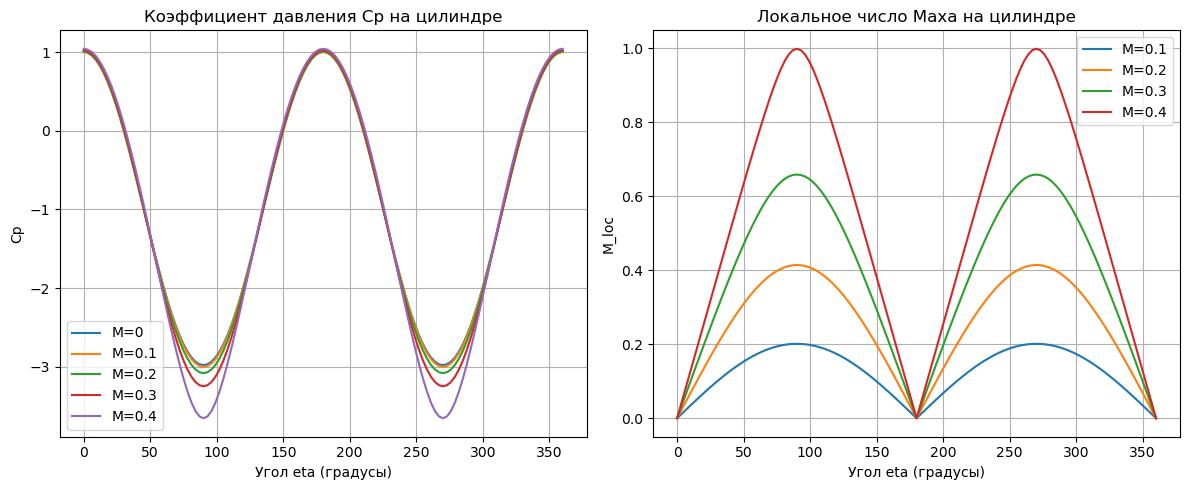
\includegraphics[width=0.9\textwidth]{../SLOP/output.png}
    \caption{Результаты расчета методом SLOR: распределение $C_p$ и $M_{loc}$ на поверхности цилиндра}
    \label{fig:slor_results}
\end{figure}

\begin{figure}[H]
    \centering
    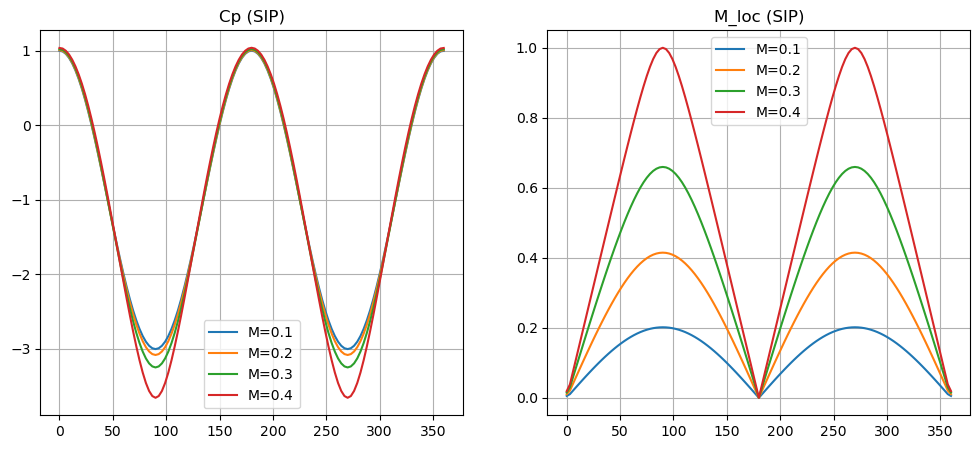
\includegraphics[width=0.9\textwidth]{../PNM (SIP)/output.png}
    \caption{Результаты расчета методом SIP (PNM): распределение $C_p$ и $M_{loc}$ на поверхности цилиндра}
    \label{fig:sip_results}
\end{figure}

\subsection{Сравнительный анализ методов}

В таблице \ref{tab:comparison} приведены значения характеристик потока в критической точке цилиндра ($\eta = \pi/2$, верхняя точка) и количество итераций, потребовавшееся для сходимости каждого метода.

\begin{table}[H]
    \centering
    \caption{Сравнение результатов методов SIP (PNM) и SLOR в точке $\eta = \pi/2$}
    \label{tab:comparison}
    \begin{tabular}{@{}ccccccc@{}}
        \toprule
        $M_\infty$ & \multicolumn{3}{c}{ПНМ (SIP)} & \multicolumn{3}{c}{SLOR} \\
        \cmidrule(lr){2-4} \cmidrule(lr){5-7}
                   & $M_{loc}$ & $C_p$ & Итерации & $M_{loc}$ & $C_p$ & Итерации \\
        \midrule
        0.1        & 0.2013    & -3.0040 & 903      & 0.2012    & -3.0023 & 225      \\
        0.2        & 0.4144    & -3.0831 & 272      & 0.4143    & -3.0816 & 325      \\
        0.3        & 0.6591    & -3.2504 & 328      & 0.6589    & -3.2484 & 400      \\
        0.4        & 0.9993    & -3.6577 & 432      & 0.9988    & -3.6547 & 520      \\
        \bottomrule
    \end{tabular}
\end{table}

\subsection{Заключение по результатам}

Проведенные расчеты позволяют сделать следующие выводы:
\begin{enumerate}
    \item Оба метода (SLOR и SIP) показывают высокую степень согласия в результатах расчета физических величин ($C_p$ и $M_{loc}$). Различия в значениях пренебрежимо малы и обусловлены особенностями численной реализации.
    \item С ростом числа Маха набегающего потока $M_\infty$ наблюдается закономерное увеличение локальной скорости и уменьшение коэффициента давления в окрестности верхней точки цилиндра. При $M_\infty = 0.4$ поток становится практически звуковым в критической области ($M_{loc} \approx 1$).
    \item Метод SIP (Полностью Неявный Метод) при малых числах Маха ($M=0.1$) требует большего числа итераций при старте с невозмущенного поля, однако при наличии хорошего начального приближения (последовательный расчет по Mach) показывает скорость сходимости, сопоставимую с методом SLOR.
    \item Метод SLOR стабильно сходится за умеренное число итераций во всем диапазоне дозвуковых скоростей, подтверждая свою эффективность для задач потенциального обтекания.
\end{enumerate}

\newpage

	
	\appendix
\section{Приложение: Вывод уравнения в координатах \texorpdfstring{$(\xi, \eta)$}{(xi, eta)}}	
Уравнение неразрывности в полярных координатах:
\[
\frac{1}{r} \frac{\partial}{\partial r} \left( \rho r \frac{\partial \varphi}{\partial r} \right) + \frac{1}{r^2} \frac{\partial}{\partial \theta} \left( \rho \frac{\partial \varphi}{\partial \theta} \right) = 0.
\]
Переходя к переменным $(\xi, \eta)$ с учетом $\frac{\partial}{\partial r} = e^{-\xi} \frac{\partial}{\partial \xi}$, $\frac{\partial}{\partial \theta} = \frac{\partial}{\partial \eta}$, $r = e^{\xi}$:
\[
\frac{\partial}{\partial \xi} \left( \rho \frac{\partial \varphi}{\partial \xi} \right) + \frac{\partial}{\partial \eta} \left( \rho \frac{\partial \varphi}{\partial \eta} \right) = 0.
\]


\section{Вывод коэффициентов пятиточечного шаблона для ПНМ}

В полностью неявном методе (ПНМ) уравнение неразрывности решается одновременно для всей области. Для этого в каждом узле $(i, j)$ записывается дискретный аналог уравнения в виде невязки $F_{i, j} = 0$.

\subsection{Дискретизация и линеаризация}

Используя центральные разности для потоков (аналогично разделу \ref{sec:slor_derivation}), запишем значение невязки в узле $(i, j)$:
\[
F_{i,j} = \frac{\rho_{i+1/2,j}(\varphi_{i+1,j} - \varphi_{i,j}) - \rho_{i-1/2,j}(\varphi_{i,j} - \varphi_{i-1,j})}{\Delta \xi^2} + \frac{\rho_{i,j+1/2}(\varphi_{i,j+1} - \varphi_{i,j}) - \rho_{i,j-1/2}(\varphi_{i,j} - \varphi_{i,j-1})}{\Delta \eta^2}
\]
Для решения нелинейной системы методом замороженной плотности ищется поправка $\delta\varphi$, такая что:
\[
\frac{\partial F_{i,j}}{\partial \varphi} \delta\varphi = -F_{i,j}
\]
В предположении «замороженной» плотности ($\rho \approx \text{const}$ на шаге итерации), это приводит к пятиточечному уравнению:
\[
\hat{A}_{i,j} \delta \varphi_{i,j-1} + A_{i,j} \delta \varphi_{i-1,j} + B_{i,j} \delta \varphi_{i,j} + C_{i,j} \delta \varphi_{i+1,j} + \hat{C}_{i,j} \delta \varphi_{i,j+1} = -F_{i,j}
\]

\subsection{Коэффициенты матрицы ПНМ}

Сравнивая невязку с общим видом пятиточечной схемы, получаем формулы для коэффициентов:
\begin{itemize}
	\item $A_{i,j} = \displaystyle \frac{\rho_{i-1/2,j}}{\Delta \xi^2}$ — связь с левым узлом ($i-1$).
	\item $C_{i,j} = \displaystyle \frac{\rho_{i+1/2,j}}{\Delta \xi^2}$ — связь с правым узлом ($i+1$).
	\item $\hat{A}_{i,j} = \displaystyle \frac{\rho_{i,j-1/2}}{\Delta \eta^2}$ — связь с нижним узлом ($j-1$).
	\item $\hat{C}_{i,j} = \displaystyle \frac{\rho_{i,j+1/2}}{\Delta \eta^2}$ — связь с верхним узлом ($j+1$).
	\item $B_{i,j} = \displaystyle -\left( \frac{\rho_{i+1/2,j} + \rho_{i-1/2,j}}{\Delta \xi^2} + \frac{\rho_{i,j+1/2} + \rho_{i,j-1/2}}{\Delta \eta^2} \right)$ — центральный коэффициент.
\end{itemize}

Данная система уравнений имеет пятидиагональную структуру и решается в данной работе с помощью сильно неявной процедуры (SIP) Стоуна.

\section{Вывод коэффициентов трехдиагональной системы метода SLOR}
\label{sec:slor_derivation}

Для численного решения уравнения неразрывности:
\[
\frac{\partial}{\partial \xi} \left( \rho \frac{\partial \varphi}{\partial \xi} \right) + \frac{\partial}{\partial \eta} \left( \rho \frac{\partial \varphi}{\partial \eta} \right) = 0
\]
используется аппроксимация центральными разностями второго порядка в узле $(i, j)$.

\subsection{Дискретизация потоков}

Поток через правую грань контрольного объема ($i+1/2, j$):
\[
\left( \rho \frac{\partial \varphi}{\partial \xi} \right)_{i+1/2, j} \approx \rho_{i+1/2, j} \frac{\varphi_{i+1, j} - \varphi_{i, j}}{\Delta \xi}
\]
Поток через левую грань ($i-1/2, j$):
\[
\left( \rho \frac{\partial \varphi}{\partial \xi} \right)_{i-1/2, j} \approx \rho_{i-1/2, j} \frac{\varphi_{i, j} - \varphi_{i-1, j}}{\Delta \xi}
\]
Аналогично для направлений по $\eta$:
\[
\left( \rho \frac{\partial \varphi}{\partial \eta} \right)_{i, j+1/2} \approx \rho_{i, j+1/2} \frac{\varphi_{i, j+1} - \varphi_{i, j}}{\Delta \eta}, \quad \left( \rho \frac{\partial \varphi}{\partial \eta} \right)_{i, j-1/2} \approx \rho_{i, j-1/2} \frac{\varphi_{i, j} - \varphi_{i, j-1}}{\Delta \eta}
\]

\subsection{Формирование системы уравнений}

Подставляя аппроксимации в уравнение и умножая на $-1$, получим:
\[
\frac{\rho_{i-1/2,j}(\varphi_{i,j} - \varphi_{i-1,j}) - \rho_{i+1/2,j}(\varphi_{i+1,j} - \varphi_{i,j})}{\Delta \xi^2} + \frac{\rho_{i,j-1/2}(\varphi_{i,j} - \varphi_{i,j-1}) - \rho_{i,j+1/2}(\varphi_{i,j+1} - \varphi_{i,j})}{\Delta \eta^2} = 0
\]
Группируя слагаемые при неизвестных на текущей строке $j$ ($\varphi_{i-1,j}, \varphi_{i,j}, \varphi_{i+1,j}$):
\[
A_i \varphi_{i-1,j} + B_i \varphi_{i,j} + C_i \varphi_{i+1,j} = D_i
\]
где коэффициенты определяются как:
\begin{itemize}
	\item $A_i = \displaystyle \frac{\rho_{i-1/2,j}}{\Delta \xi^2}$ — влияние предыдущего узла.
	\item $C_i = \displaystyle \frac{\rho_{i+1/2,j}}{\Delta \xi^2}$ — влияние следующего узла.
	\item $B_i = \displaystyle -\left( \frac{\rho_{i+1/2,j} + \rho_{i-1/2,j}}{\Delta \xi^2} + \frac{\rho_{i,j+1/2} + \rho_{i,j-1/2}}{\Delta \eta^2} \right)$ — центральный коэффициент.
	\item $D_i = \displaystyle - \frac{\rho_{i,j+1/2} \varphi_{i,j+1} + \rho_{i,j-1/2} \varphi_{i,j-1}}{\Delta \eta^2}$ — вклад соседних строк.
\end{itemize}

Данный вид системы обеспечивает выполнение принципа максимума и диагональное преобладание ($|B_i| = A_i + C_i + \text{положительные члены}$), что гарантирует устойчивость и сходимость итерационного процесса.

	\section{Алгоритм численного решения задачи обтекания цилиндра}

В данном разделе приведено пошаговое описание численного алгоритма, реализованного для моделирования дозвукового обтекания цилиндра. Алгоритм базируется на итерационном методе последовательной верхней релаксации по линиям (SLOR).

\subsection{Входные данные и параметры расчета}

Перед началом расчета задаются следующие физические и численные параметры:
\begin{itemize}
    \item $M_\infty$ --- число Маха набегающего потока;
    \item $\gamma = 1.4$ --- показатель адиабаты для воздуха;
    \item $\omega$ --- параметр верхней релаксации (подбирается экспериментально, обычно $1.5 < \omega < 1.8$);
    \item $\epsilon$ --- требуемая точность расчета (критерий остановки по максимальной невязке).
\end{itemize}

\subsection{Генерация расчетной сетки}

Для эффективного решения задачи используется конформное отображение, переводящее внешность цилиндра в полуполосу в плоскости криволинейных координат $(\xi, \eta)$.

\begin{enumerate}
    \item Задается число узлов по радиальной координате $N_\xi$ и по углу $N_\eta$.
    \item Вычисляются шаги сетки: $h_\xi = \xi_{max} / N_\xi$, $h_\eta = 2\pi / N_\eta$.
    \item Связь с физическими координатами $(x, y)$ осуществляется по формулам:
    \[ x_{i,j} = e^{\xi_i} \cos \eta_j, \quad y_{i,j} = e^{\xi_i} \sin \eta_j \]
\end{enumerate}
Такое преобразование позволяет получить сетку, узлы которой сгущаются по экспоненциальному закону при приближении к поверхности цилиндра ($\xi=0$), что критически важно для корректного разрешения больших градиентов параметров.

\subsection{Начальное приближение и граничные условия}

В качестве начального распределения потенциала $\varphi^0$ используется аналитическое решение для обтекания цилиндра несжимаемой жидкостью:
\[ \varphi_{i,j}^0 = (e^{\xi_i} + e^{-\xi_i})\cos\eta_j \]

Граничные условия ставятся следующим образом:
\begin{itemize}
    \item \textbf{На внешней границе} ($\xi = \xi_{max}$): фиксируется потенциал невозмущенного потока (условие Дирихле):
    \[ \varphi_{N_\xi, j} = e^{\xi_{max}} \cos \eta_j \]
    \item \textbf{На поверхности цилиндра} ($\xi = 0$): ставится условие непротекания (условие Неймана):
    \[ \frac{\partial \varphi}{\partial \xi} = 0 \]
    \item \textbf{На линиях $\eta=0$ и $\eta=2\pi$}: используются условия симметрии потока.
\end{itemize}

\subsection{Итерационный процесс решения}

Расчет продолжается до тех пор, пока не будет выполнено условие сходимости:
\[ \max_{i,j} \left| \varphi_{i,j}^{k+1} - \varphi_{i,j}^k \right| < \epsilon \]

Каждая итерация включает в себя два основных этапа:

\subsubsection{Обновление поля плотности}
На основе значений потенциала с предыдущего шага вычисляются компоненты скорости и плотность в каждом узле:
\begin{enumerate}
    \item Производные потенциала в узлах:
    \[ \varphi_\xi \approx \frac{\varphi_{i+1,j} - \varphi_{i-1,j}}{2h_\xi}, \quad \varphi_\eta \approx \frac{\varphi_{i,j+1} - \varphi_{i,j-1}}{2h_\eta} \]
    \item Квадрат модуля скорости:
    \[ q_{i,j}^2 = e^{-2\xi_i} \left( \varphi_\xi^2 + \varphi_\eta^2 \right) \]
    \item Локальная плотность $\rho$ по закону Бернулли для сжимаемого газа:
    \[ \rho_{i,j} = \left[1 + \frac{\gamma-1}{2} M_\infty^2 (1 - q_{i,j}^2)\right]^{\frac{1}{\gamma-1}} \]
\end{enumerate}

\subsubsection{Решение уравнения для потенциала (SLOR)}
Уравнение неразрывности решается итерационным методом по радиальным линиям (кольцам). Для каждой линии $j = \text{const}$ решается трехдиагональная система уравнений 

\[A_i \varphi_{i-1,j}^* + B_i \varphi_{i,j}^* + C_i \varphi_{i+1,j}^* = D_i\].

Коэффициенты матрицы вычисляются с использованием плотностей на гранях ячеек:
\[ A_i = -\frac{\rho_{i-1/2, j}}{h_\xi^2}, \quad C_i = -\frac{\rho_{i+1/2, j}}{h_\xi^2} \]
\[ B_i = \frac{\rho_{i-1/2, j} + \rho_{i+1/2, j}}{h_\xi^2} + \frac{\rho_{i, j-1/2} + \rho_{i, j+1/2}}{h_\eta^2} \]
\[ D_i = \frac{\rho_{i, j-1/2} \varphi_{i, j-1}^{k+1} + \rho_{i, j+1/2} \varphi_{i, j+1}^k}{h_\eta^2} \]

После решения системы методом прогонки применяется процедура верхней релаксации:
\[ \varphi_{i,j}^{k+1} = \varphi_{i,j}^k + \omega \left( \varphi_{i,j}^* - \varphi_{i,j}^k \right) \]


\end{document}
